%%%%%%%%%%%%%%%%%%%%%%%%%%%%%%%%%%%%%%%%%%%%%%%%%%%%%%%%%%%%%%%%%%%%%%%%%%%%%%%%%%
\section{Intro}
%%%%%%%%%%%%%%%%%%%%%%%%%%%%%%%%%%%%%%%%%%%%%%%%%%%%%%%%%%%%%%%%%%%%%%%%%%%%%%%%%%

\begin{frame}{Vorstellung}
	\begin{block}{Punkte}
		\begin{itemize}
			\item Fachgebiet
			\item Konkrete Erwartungen an den Kurs
			\item `Bitte-nicht'-Erwartungen
			\item Interesse an bestimmer Sprachfamilie
		\end{itemize}
	\end{block}
\end{frame}
%%%%%%%%%%%%%%%%%%%%%%%%%%%%%%%%%%%%%%%%%%%%%%%%%%%%%%%%%%%%%%%%%%%%%%%%%%%%%%%%%%


%%%%%%%%%%%%%%%%%%%%%%%%%%%%%%%%%%%%%%%%%%%%%%%%%%%%%%%%%%%%%%%%%%%%%%%%%%%%%%%%%%
\begin{frame}{Inhalt}
	\begin{block}{Überblick}
		\begin{itemize}
			\item Erstellung eines Lexibank-datasets (Digitalisierung von Daten)
			\item Annotation der Daten in EDICTOR
			\item Manuelle Auswertung der Annotation
			\item Automatisierte Auswertung der Annotation
		\end{itemize}
	\end{block}
\end{frame}
%%%%%%%%%%%%%%%%%%%%%%%%%%%%%%%%%%%%%%%%%%%%%%%%%%%%%%%%%%%%%%%%%%%%%%%%%%%%%%%%%%


%%%%%%%%%%%%%%%%%%%%%%%%%%%%%%%%%%%%%%%%%%%%%%%%%%%%%%%%%%%%%%%%%%%%%%%%%%%%%%%%%%
\section{Historische Linguistik}
%%%%%%%%%%%%%%%%%%%%%%%%%%%%%%%%%%%%%%%%%%%%%%%%%%%%%%%%%%%%%%%%%%%%%%%%%%%%%%%%%%
%%%%%%%%%%%%%%%%%%%%%%%%%%%%%%%%%%%%%%%%%%%%%%%%%%%%%%%%%%%%%%%%%%%%%%%%%%%%%%%%%%
\begin{frame}{Große Sprachfamilien der Welt}
%%%%%%%%%%%%%%%%%%%%%%%%%%%%%%%%%%%%%%%%%%%%%%%%%%%%%%%%%%%%%%%%%%%%%%%%%%%%%%%%%%
	\begin{itemize}
		\item $\sim$7000 Sprachen weltweit
		\item Indo-Europäisch: \url{https://glottolog.org/resource/languoid/id/indo1319}
		\item Austronesisch: \url{https://glottolog.org/resource/languoid/id/aust1307}
		\item Arawak: \url{https://glottolog.org/resource/languoid/id/araw1281}
		\item Bantu: \url{https://glottolog.org/resource/languoid/id/narr1281}
	\end{itemize}
\end{frame}
%%%%%%%%%%%%%%%%%%%%%%%%%%%%%%%%%%%%%%%%%%%%%%%%%%%%%%%%%%%%%%%%%%%%%%%%%%%%%%%%%%

%%%%%%%%%%%%%%%%%%%%%%%%%%%%%%%%%%%%%%%%%%%%%%%%%%%%%%%%%%%%%%%%%%%%%%%%%%%%%%%%%%
\begin{frame}{Ähnlichkeiten zwischen Wörtern: Woher und wieso?}
%%%%%%%%%%%%%%%%%%%%%%%%%%%%%%%%%%%%%%%%%%%%%%%%%%%%%%%%%%%%%%%%%%%%%%%%%%%%%%%%%%
	\begin{itemize}
		\pause
		\item Zufall, Kontakt, Verwandtschaft
		\pause
		\item Beispiele aus etymologischen Wörterbuch für Sprachwandel? \pause
	\end{itemize}
	\begin{figure}
		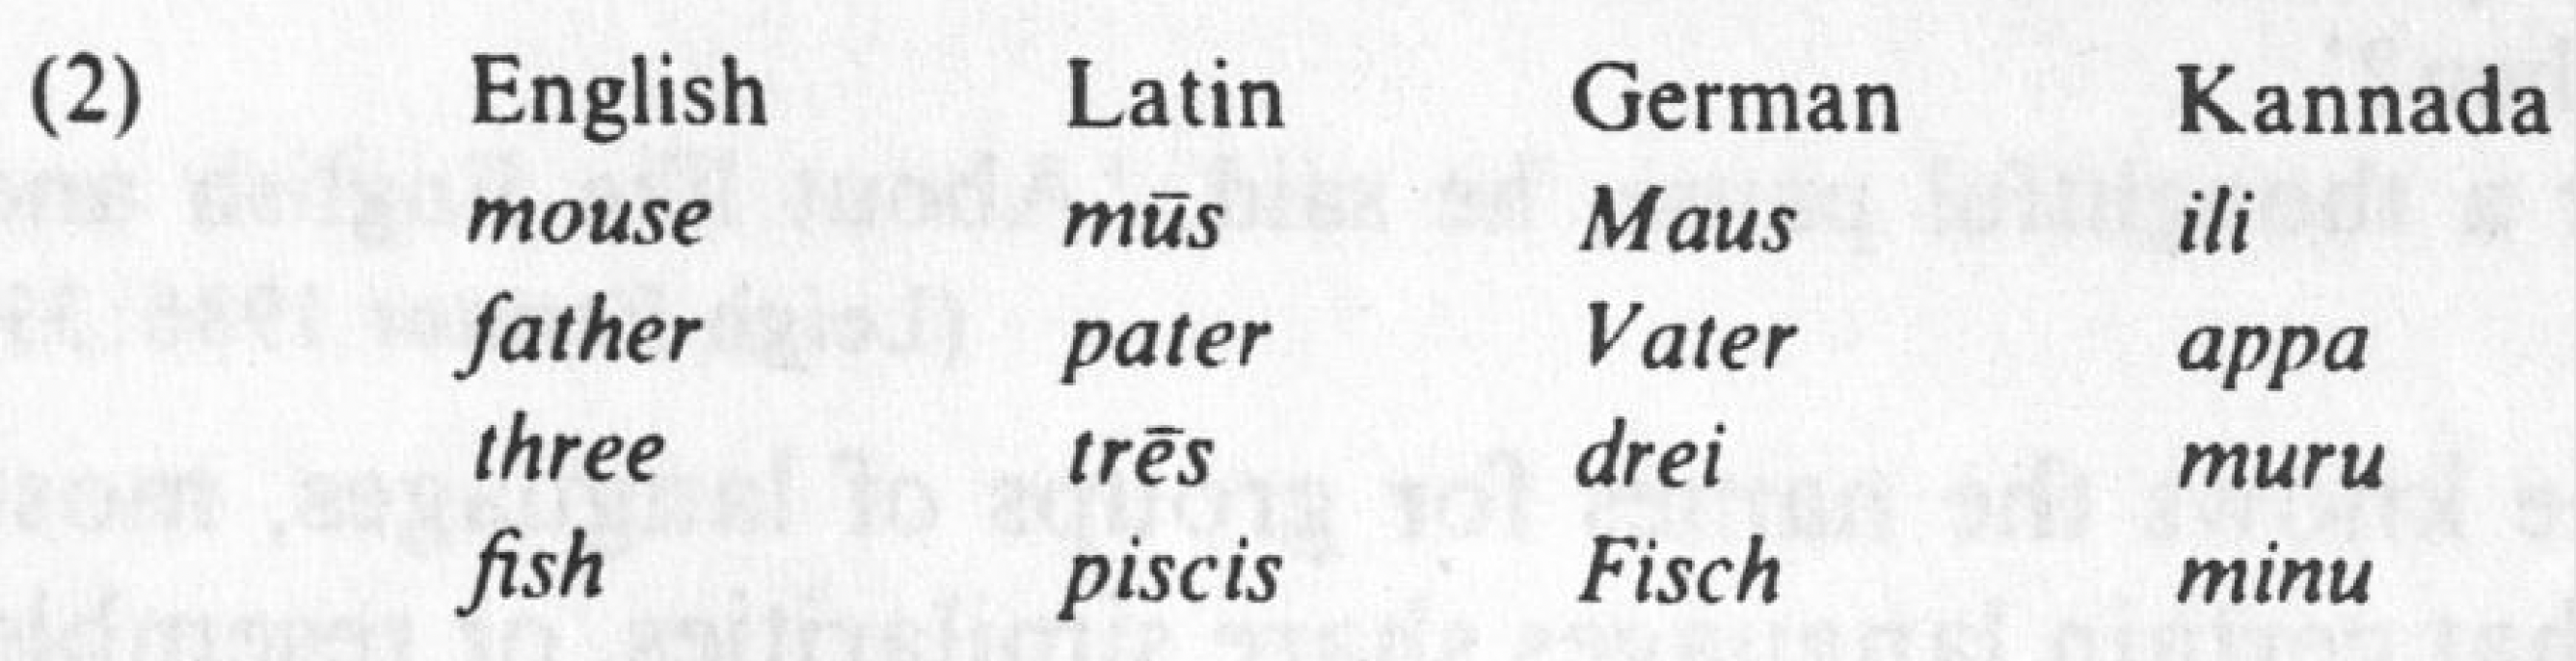
\includegraphics[height=0.3\textheight]{images/ie_korrespondenzen.png}
		\caption{Verwandte Wörter in Indo-Europäischen Sprachen \parencite{McMahon1994}}
	\end{figure}
\end{frame}
%%%%%%%%%%%%%%%%%%%%%%%%%%%%%%%%%%%%%%%%%%%%%%%%%%%%%%%%%%%%%%%%%%%%%%%%%%%%%%%%%%
		


%%%%%%%%%%%%%%%%%%%%%%%%%%%%%%%%%%%%%%%%%%%%%%%%%%%%%%%%%%%%%%%%%%%%%%%%%%%%%%%%%%
\begin{frame}{Ähnlichkeiten zwischen Wörtern: Zufall}
%%%%%%%%%%%%%%%%%%%%%%%%%%%%%%%%%%%%%%%%%%%%%%%%%%%%%%%%%%%%%%%%%%%%%%%%%%%%%%%%%%
	\begin{itemize}
		\item Manche Formen sind nur aus Zufall ähnlich
	\end{itemize}
	\begin{figure}
		\includegraphics[height=0.2\textheight]{images/zufälle.png}
		\caption{Wörter mit ähnlichen Formen und Bedeutungen in nicht-verwandten Sprachen \parencite{McMahon1994}}
	\end{figure}
\end{frame}
%%%%%%%%%%%%%%%%%%%%%%%%%%%%%%%%%%%%%%%%%%%%%%%%%%%%%%%%%%%%%%%%%%%%%%%%%%%%%%%%%%
	

%%%%%%%%%%%%%%%%%%%%%%%%%%%%%%%%%%%%%%%%%%%%%%%%%%%%%%%%%%%%%%%%%%%%%%%%%%%%%%%%%%
\begin{frame}{Ähnlichkeiten zwischen Wörtern: Kontakt}
%%%%%%%%%%%%%%%%%%%%%%%%%%%%%%%%%%%%%%%%%%%%%%%%%%%%%%%%%%%%%%%%%%%%%%%%%%%%%%%%%%
	\begin{itemize}
		\item *vinum (Latein) > Wein/vine
		\item *strata (Latein) > Straße/street
	\end{itemize}
\end{frame}
%%%%%%%%%%%%%%%%%%%%%%%%%%%%%%%%%%%%%%%%%%%%%%%%%%%%%%%%%%%%%%%%%%%%%%%%%%%%%%%%%%

%%%%%%%%%%%%%%%%%%%%%%%%%%%%%%%%%%%%%%%%%%%%%%%%%%%%%%%%%%%%%%%%%%%%%%%%%%%%%%%%%%
\begin{frame}{Ähnlichkeiten zwischen Wörtern: Verwandtschaft}
%%%%%%%%%%%%%%%%%%%%%%%%%%%%%%%%%%%%%%%%%%%%%%%%%%%%%%%%%%%%%%%%%%%%%%%%%%%%%%%%%%
	\begin{itemize}
		\item Verbindung zwischen Form und Bedeutung ist (meistens) arbiträr  \pause
		\item Evaluation regelmäßiger Lautkorrespondenzen zwischen Sprachen als Evidenz für gemeinsame Abstammung
	\end{itemize}
\end{frame}
%%%%%%%%%%%%%%%%%%%%%%%%%%%%%%%%%%%%%%%%%%%%%%%%%%%%%%%%%%%%%%%%%%%%%%%%%%%%%%%%%%


%%%%%%%%%%%%%%%%%%%%%%%%%%%%%%%%%%%%%%%%%%%%%%%%%%%%%%%%%%%%%%%%%%%%%%%%%%%%%%%%%%
%%%%%%%%%%%%%%%%%%%%%%%%%%%%%%%%%%%%%%%%%%%%%%%%%%%%%%%%%%%%%%%%%%%%%%%%%%%%%%%%%%
\begin{frame}{Junggrammatiker}
%%%%%%%%%%%%%%%%%%%%%%%%%%%%%%%%%%%%%%%%%%%%%%%%%%%%%%%%%%%%%%%%%%%%%%%%%%%%%%%%%%
	\begin{itemize}
		\item Eine Gruppe junger Forscher in Leipzig
		\item Systematische und wissenschaftliche Untersuchung des Sprachwandels nach strengen methodologischen Kriterien, die bis heute halten
		\item Vorher: Oft Referenz auf `Urform' der Sprache, welche verunstaltet wird durch Wandel
	\end{itemize}
		\pause
		\begin{block}{Regularitätsprinzip}
			\begin{itemize}
			\item Regularitätsprinzip: Aller Lautwandel ist regelmäßig
			\item Operationalisiert: Es ist dann Lautwandel, wenn es regelmäßig ist \parencite{Hoenigswald1978}
		\end{itemize}
	\end{block} 
\end{frame}
%%%%%%%%%%%%%%%%%%%%%%%%%%%%%%%%%%%%%%%%%%%%%%%%%%%%%%%%%%%%%%%%%%%%%%%%%%%%%%%%%%

%%%%%%%%%%%%%%%%%%%%%%%%%%%%%%%%%%%%%%%%%%%%%%%%%%%%%%%%%%%%%%%%%%%%%%%%%%%%%%%%%%
\begin{frame}{Regularitätsprinzip: Und jetzt?}
%%%%%%%%%%%%%%%%%%%%%%%%%%%%%%%%%%%%%%%%%%%%%%%%%%%%%%%%%%%%%%%%%%%%%%%%%%%%%%%%%%
\begin{block}{Kognate}
	\begin{itemize}
		\item Wörter die regelmäßige und wiederholte Lautkorrespondenzen zwischen mehreren Sprachen sowie eine ähnliche Bedeutung zeigen
		\pause
		\item Annahme: Die Wörter haben einen gemeinsamen `Vorfahren'
	\end{itemize}
\end{block}

\begin{block}{Sprachfamilien}
	\begin{itemize}
		\item Verwandte Sprachen waren einmal die \textit{gleiche} Sprache (Proto-Sprache)
		\item Beispiel: Proto-Indo-Europäisch
	\end{itemize}
\end{block}
\end{frame}
%%%%%%%%%%%%%%%%%%%%%%%%%%%%%%%%%%%%%%%%%%%%%%%%%%%%%%%%%%%%%%%%%%%%%%%%%%%%%%%%%%


%%%%%%%%%%%%%%%%%%%%%%%%%%%%%%%%%%%%%%%%%%%%%%%%%%%%%%%%%%%%%%%%%%%%%%%%%%%%%%%%%%
\begin{frame}{Rekonstruktionen}
%%%%%%%%%%%%%%%%%%%%%%%%%%%%%%%%%%%%%%%%%%%%%%%%%%%%%%%%%%%%%%%%%%%%%%%%%%%%%%%%%%
\begin{itemize}
	\item Rekonstruktion vorhergehender Sprachstufen (markiert mit Asterisk `*')
	\item Ableitung von Lautwandel-`Gesetzen' \pause
	\item Beispiele: 
	\begin{itemize}
		\item *k > h zwischen Vokalen in Tacana und Warisa
		\item *u > o in Ese Ejja
	\end{itemize}
\end{itemize}
	\begin{table}
		\begin{tabular}[pos]{|l|c|c|c|c|}
			\hline
			Proto-Takana	& d	& u	& k	& u \\ \hline
			Kaviñena		& d	& u	& k	& u \\
			Tacana			& d	& u	& h	& u \\
			Warisa			& d	& o	& h	& o \\
			Ese	Ejja		& d	& o	& x	& o \\
			\hline
		\end{tabular}
		\caption{Wörter für \textsc{INNEN} in verschiedenen Takana-Sprachen \parencite{Girard1971}}
	\end{table}
\end{frame}
%%%%%%%%%%%%%%%%%%%%%%%%%%%%%%%%%%%%%%%%%%%%%%%%%%%%%%%%%%%%%%%%%%%%%%%%%%%%%%%%%%

%%%%%%%%%%%%%%%%%%%%%%%%%%%%%%%%%%%%%%%%%%%%%%%%%%%%%%%%%%%%%%%%%%%%%%%%%%%%%%%%%%
%%%%%%%%%%%%%%%%%%%%%%%%%%%%%%%%%%%%%%%%%%%%%%%%%%%%%%%%%%%%%%%%%%%%%%%%%%%%%%%%%%
\begin{frame}{Phonologische Klassifizierung von Lautwandel}
%%%%%%%%%%%%%%%%%%%%%%%%%%%%%%%%%%%%%%%%%%%%%%%%%%%%%%%%%%%%%%%%%%%%%%%%%%%%%%%%%%
	\begin{block}{Lautinventar der Sprache}
		\begin{itemize}
			\item Merge: Zwei Laute verbinden sich zu einem (*m und *n werden zu /n/) \pause
			\item Split: Ein Laut wird zu zwei Lauten
			\begin{itemize}
				\item Oft eine kontextabhängige Variation
				\item Beispiel: /n/ vor /p/ wird /m/, aber bleibt /n/ in allen anderen Fällen \pause
				\item Secondary Split: Neuer Laut im Inventar der Sprache
				\item Primary split: `Merge' mit anderem Laut
			\end{itemize}
			\item Shift: Isolierter Lautwandel, ohne Merge/Split
		\end{itemize}
	\end{block}
\end{frame}
%%%%%%%%%%%%%%%%%%%%%%%%%%%%%%%%%%%%%%%%%%%%%%%%%%%%%%%%%%%%%%%%%%%%%%%%%%%%%%%%%%


%%%%%%%%%%%%%%%%%%%%%%%%%%%%%%%%%%%%%%%%%%%%%%%%%%%%%%%%%%%%%%%%%%%%%%%%%%%%%%%%%%
\section{CLDF}
%%%%%%%%%%%%%%%%%%%%%%%%%%%%%%%%%%%%%%%%%%%%%%%%%%%%%%%%%%%%%%%%%%%%%%%%%%%%%%%%%%
\begin{frame}{CLDF}
%%%%%%%%%%%%%%%%%%%%%%%%%%%%%%%%%%%%%%%%%%%%%%%%%%%%%%%%%%%%%%%%%%%%%%%%%%%%%%%%%%
\begin{block}{Referenzkataloge}
	\begin{itemize}
		\item \href{https://glottolog.org/}{Glottolog}
		\item \href{https://concepticon.clld.org/}{Concepticon}
		\item \href{https://clts.clld.org/}{CLTS}
	\end{itemize}
\end{block}
\end{frame}
%%%%%%%%%%%%%%%%%%%%%%%%%%%%%%%%%%%%%%%%%%%%%%%%%%%%%%%%%%%%%%%%%%%%%%%%%%%%%%%%%%

%%%%%%%%%%%%%%%%%%%%%%%%%%%%%%%%%%%%%%%%%%%%%%%%%%%%%%%%%%%%%%%%%%%%%%%%%%%%%%%%%%
\begin{frame}{CLDF}
%%%%%%%%%%%%%%%%%%%%%%%%%%%%%%%%%%%%%%%%%%%%%%%%%%%%%%%%%%%%%%%
\vspace*{-0.3cm}
	\begin{figure}
		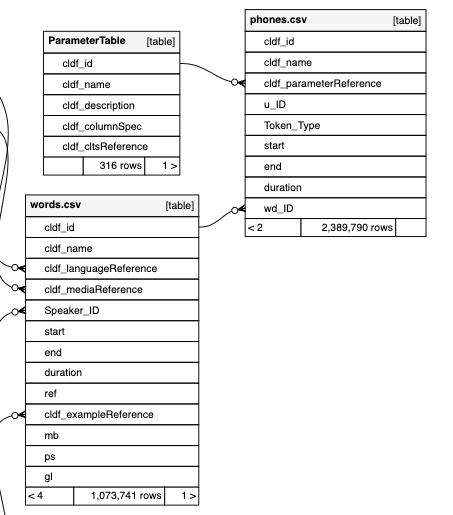
\includegraphics[height=0.75\textheight]{images/relational.png}
		\caption{CLDF als relationale Datenbanken \parencite{Forkel2018}}
	\end{figure}
\end{frame}
%%%%%%%%%%%%%%%%%%%%%%%%%%%%%%%%%%%%%%%%%%%%%%%%%%%%%%%%%%%%%%%%%%%%%%%%%%%%%%%%%%
	

%%%%%%%%%%%%%%%%%%%%%%%%%%%%%%%%%%%%%%%%%%%%%%%%%%%%%%%%%%%%%%%%%%%%%%%%%%%%%%%%%%
\section{Beispiele für Studien}
%%%%%%%%%%%%%%%%%%%%%%%%%%%%%%%%%%%%%%%%%%%%%%%%%%%%%%%%%%%%%%%%%%%%%%%%%%%%%%%%%%
\begin{frame}{Expansion der Bantu-Sprachen}
%%%%%%%%%%%%%%%%%%%%%%%%%%%%%%%%%%%%%%%%%%%%%%%%%%%%%%%%%%%%%%%%%%%%%%%%%%%%%%%%%%
\vspace*{-0.3cm}
	\begin{figure}
		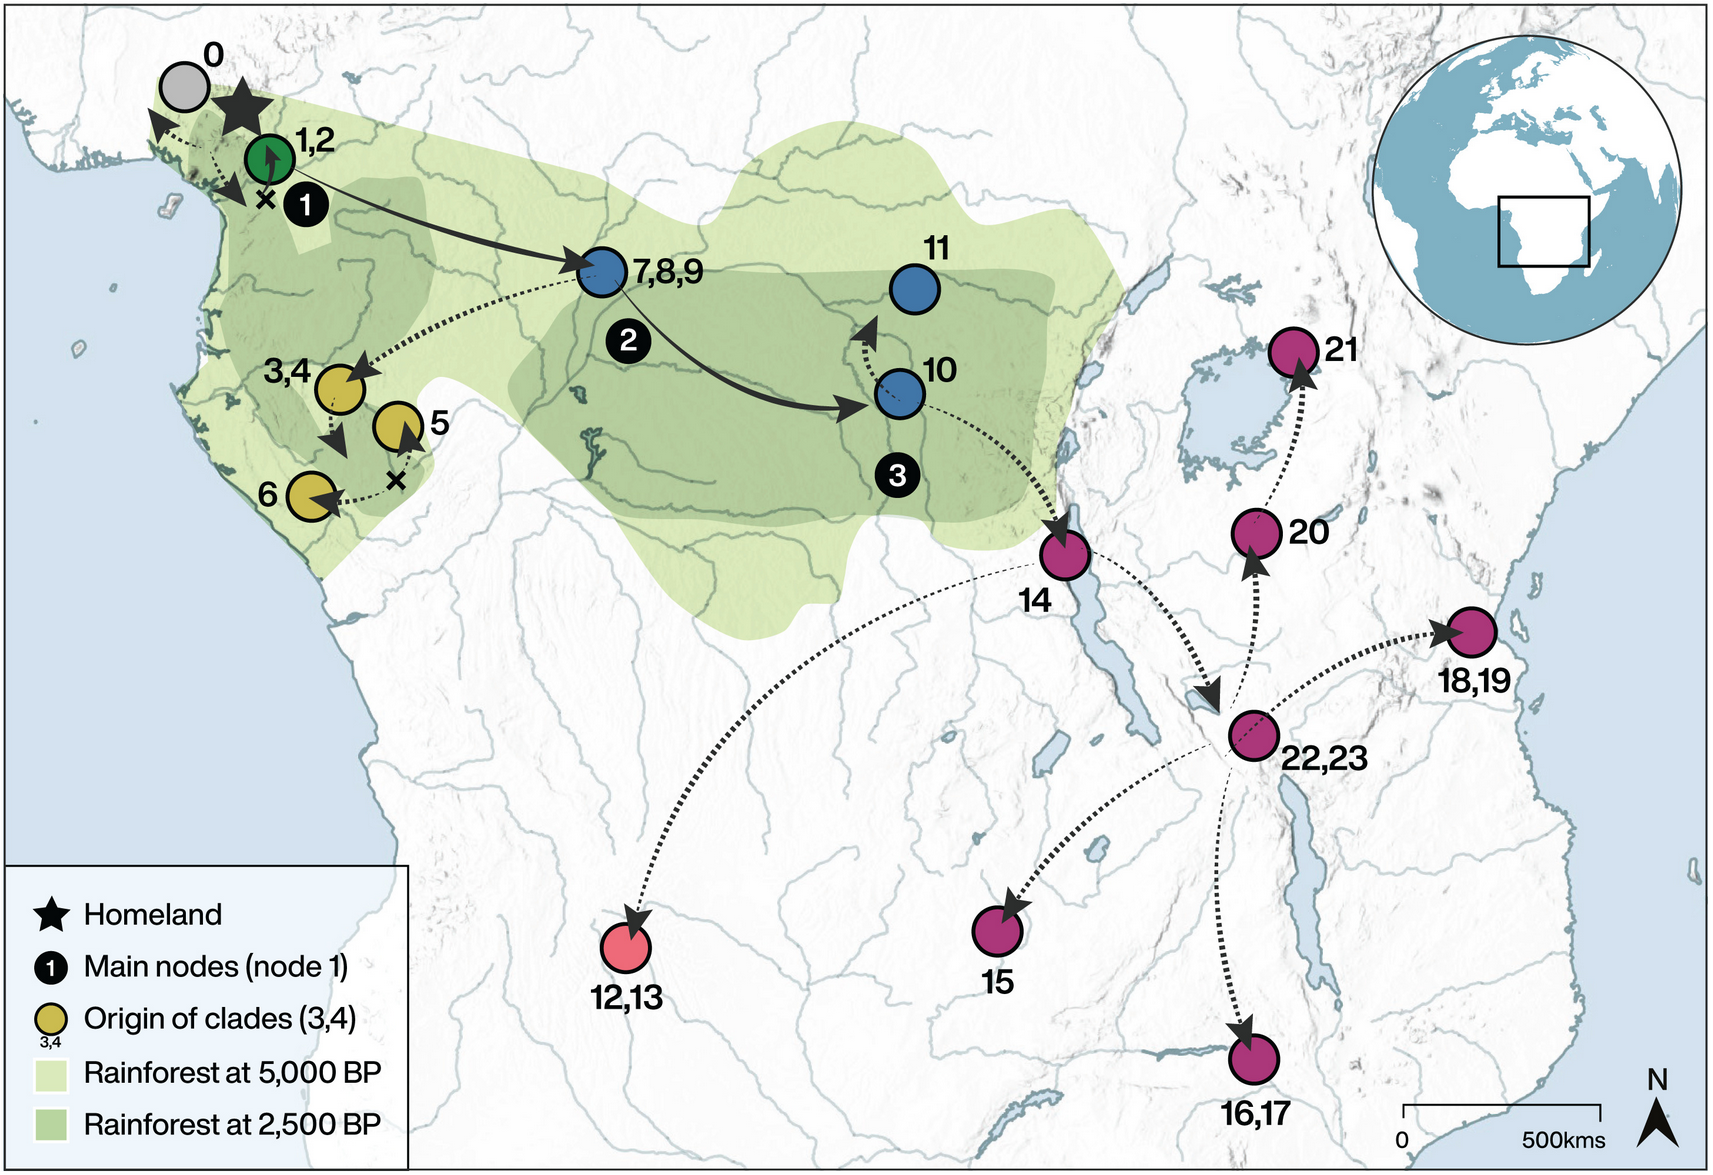
\includegraphics[height=0.75\textheight]{images/bantu.png}
		\caption{Ausbreitung der Bantu-Sprachen in Afrika \parencite{Koile2022}}
	\end{figure}
\end{frame}
%%%%%%%%%%%%%%%%%%%%%%%%%%%%%%%%%%%%%%%%%%%%%%%%%%%%%%%%%%%%%%%%%%%%%%%%%%%%%%%%%%

%%%%%%%%%%%%%%%%%%%%%%%%%%%%%%%%%%%%%%%%%%%%%%%%%%%%%%%%%%%%%%%%%%%%%%%%%%%%%%%%%%
\begin{frame}{Genetische und linguistische Evolution}
%%%%%%%%%%%%%%%%%%%%%%%%%%%%%%%%%%%%%%%%%%%%%%%%%%%%%%%%%%%%%%%%%%%%%%%%%%%%%%%%%%
\vspace*{-0.3cm}
	\begin{figure}
		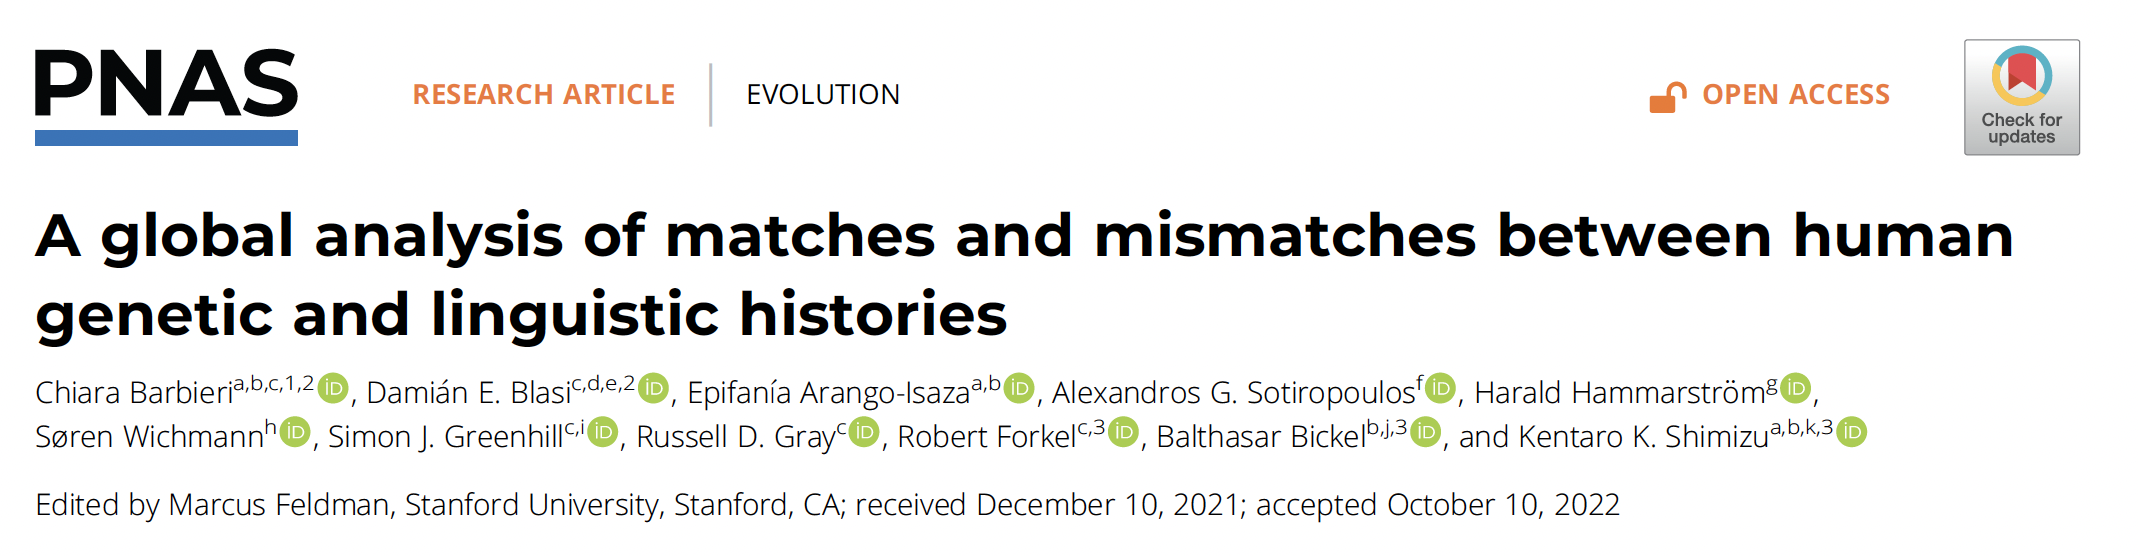
\includegraphics[width=1.1\linewidth]{images/gelato.png}
		\caption{Matches und mismatches in genetischer und linguistischer Geschichte \parencite{Barbieri2022}}
	\end{figure}
\end{frame}
%%%%%%%%%%%%%%%%%%%%%%%%%%%%%%%%%%%%%%%%%%%%%%%%%%%%%%%%%%%%%%%%%%%%%%%%%%%%%%%%%%

%%%%%%%%%%%%%%%%%%%%%%%%%%%%%%%%%%%%%%%%%%%%%%%%%%%%%%%%%%%%%%%%%%%%%%%%%%%%%%%%%%
\begin{frame}{Variation of Emotion Semantics}
%%%%%%%%%%%%%%%%%%%%%%%%%%%%%%%%%%%%%%%%%%%%%%%%%%%%%%%%%%%%%%%%%%%%%%%%%%%%%%%%%%
\vspace*{-0.3cm}
	\begin{figure}
		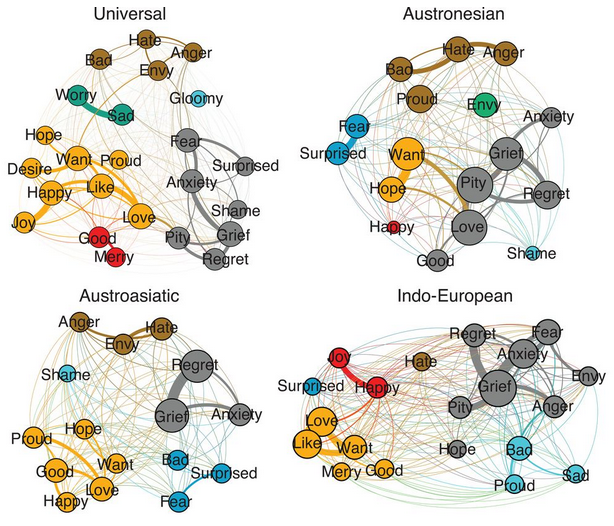
\includegraphics[height=0.75\textheight]{images/jackson.png}
		\caption{Colexification of emotion concepts \parencite{Jackson2019}}
	\end{figure}
\end{frame}
%%%%%%%%%%%%%%%%%%%%%%%%%%%%%%%%%%%%%%%%%%%%%%%%%%%%%%%%%%%%%%%%%%%%%%%%%%%%%%%%%%

	